
\documentclass[]{article}
\voffset=-1.0cm
\oddsidemargin=0.0cm
\textwidth = 480pt
\usepackage[utf8]{inputenc}
\usepackage[english]{babel}
\usepackage{framed}
\usepackage{graphicx}
\usepackage{enumerate}% http://ctan.org/pkg/enumerate
\usepackage{multicol}
\usepackage{amsmath}
\usepackage{amssymb}
\usepackage[angle=0,scale=1,color=black,hshift=-0.4cm,vshift=15cm]{background}
\usepackage{multirow}
\usepackage{eurosym}
\usepackage{vmargin}
\usepackage{amsmath}
\usepackage{graphics}
\usepackage{epsfig}
\usepackage{subfigure}
\usepackage{fancyhdr}
\usepackage{listings}
\usepackage{framed}



\begin{document}
	
	
	\subsection*{Question 5 : SPSS Output}
%	\begin{figure}[h!]
%		\centering
%		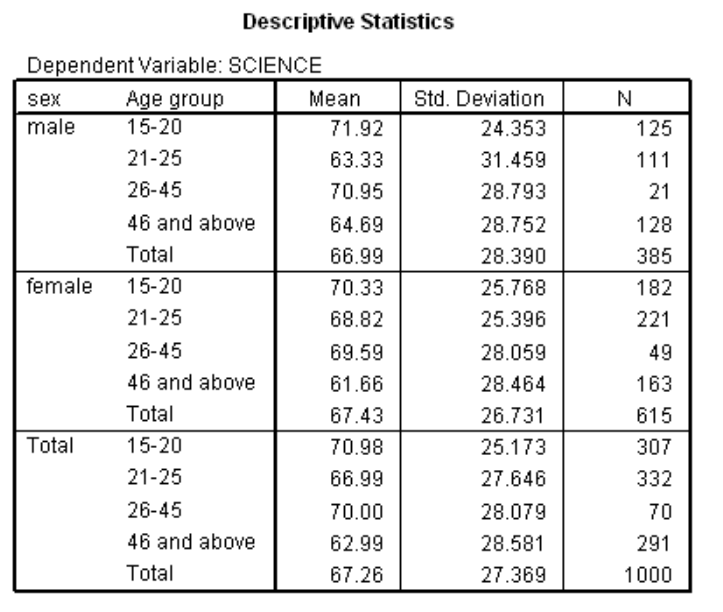
\includegraphics[width=0.65\linewidth]{images/SPSS-Week1}
%	\end{figure}
	\begin{enumerate}
		\item What is the mean Science score for all Males?
		\item What it the mean Science score for all Females?
		\item What is the mean Science score for everybody in the study?
		\item How many respondents are there altogether?
		\item How many people are in the 15-20 age group altogether?
		\item Which Age group has the highest Score?
		%	\item What is the smallest age group in the sample?
	\end{enumerate}
	
\section*{Probability Distributions}


\begin{itemize}
	\item The discrete uniform distribution
	\item The continuous uniform distribution
	\item The binomial disribution
	\item The poisson distribution
	\item The exponential distribution
	\item the Normal distribution
\end{itemize}



%\begin{enumerate}
%	%--Distributions
%	
%	
%	
%	
%	\item uniform - The lower and upper bounds are 13cm and 21cm respectively.
%	
%	\item A computer server breaks down, on average, once every three months.
	\begin{itemize}
		\item What is the probability that the server breaks down three times in a quarter?
		\item What is the probability that a server breaks down exactly five times in one year?
	\end{itemize}
	
	Assume that the number of weekly study hours for students at a certain university
	is approximately normally distributed with a mean of 22 and a standard deviation
	of 6.
	\begin{itemize}
		\item Find the probability that a randomly chosen student studies less than 12
		hours.
		\item Estimate the percentage of students that study more than 37 hours.
	\end{itemize}
	

%A charity believes that when it puts out an appeal for charitable donations the donations it receives 
%will normally distributed with a mean 50 and 
%
%standard deviation €6, and
%
% it is assumed that donations will be independent of each other.
%	
%\begin{itemize} 
%\item Find the probability that the first donation it receives will be less than€40.
%
%\item Compute the probability that it will be between €40and €45.
%\item Compute the value $x$ such that 5\% of donations are more than €$x$.
%\end{itemize}
%	
	In an examination the scores of students who attend schools of type A are
	normally distributed about a mean of 55 with a standard deviation of 6. The
	scores of students who attend type B schools are normally distributed about a
	mean of 60 with a standard deviation of 5.
	Which type of school would have a higher proportion of students with marks above 70?

The heights for a group of forty rowing club members are tabulated as follows;

\begin{table}[ht]
	\begin{center}
		\begin{tabular}{|rrrrrrrrrr|}
			
			\hline
			141 & 148 & 149 & 149 & 155 & 156 & 167 & 169 & 169 & 170 \\
			171 & 173 & 175 & 176 & 177 & 179 & 182 & 182 & 183 & 183 \\
			183 & 184 & 184 & 184 & 185 & 185 & 185 & 186 & 186 & 189 \\
			191 & 191 & 191 & 191 & 192 & 192 & 192 & 193 & 194 & 199 \\
			\hline
		\end{tabular}
	\end{center}
\end{table}
\vspace{-0.5cm}
\begin{enumerate}
	\item (6 marks) Summarize the data in the above table using a frequency table. Use 6 class intervals, with 140 as the lower limit of the first interval.
	\item (6 marks) Draw a histogram for the above data.
	\item (4 marks) Comment on the shape of the histogram. Based on the shape of the histogram, what is the best measure of centrality and variability?
	\item (12 marks) Construct a box plot for the above data. Clearly demonstrate how all of the necessary values were computed.
\end{enumerate}


\section{KB Tutorial 2}

\subsection*{Question 4}
Consider a RAID (redundant array of inexpensive disks) system where multiple hard disks are used simultaneously.\\[0.2cm]
Let's assume that we have two hard disks that work \emph{independently} of each other. Define the events $H_1 =$ ``hard disk one works'' and $H_2 =$ ``hard disk two works'' and also assume that $\Pr(H_1) = \Pr(H_2) = 0.9$.\\ \smallskip
\begin{itemize}
	\item RAID-0 is a system which increases performance but only works if \emph{both} hard disks work.
	\item RAID-1 is a system which does not increase performance but still works with only one working hard disk.
\end{itemize}

{\bf(a)} Calculate $\Pr(\text{RAID-0 works})$ and $\Pr(\text{RAID-0 fails})$. \\[0.3cm] \quad {\bf(b)} Calculate $\Pr(\text{RAID-1 works})$ and $\Pr(\text{RAID-1 fails})$. \quad {\bf(c)} Calculate $\Pr(H_1^c)$ and $\Pr(H_2^c)$. \\[0.3cm]
\quad {\bf(d)} Cheap hard disks exist with $\Pr(H) = 0.6$. Consider a RAID-1 system with 3 of these hard disks - calculate $\Pr(\text{RAID-1 fails})$ in this case. \\[0.3cm] \quad {\bf(e)} In part (a) we found that $\Pr(\text{RAID-1 fails}) = 0.01$. How many cheap disks would be required to match this level of reliability?



\subsection*{Question 5}
A software company examined blocks of code written by its employees. Each block of code was tested for bugs and, in addition, the skill level of the employee was also recorded. See table:
\begin{center}
	\begin{tabular}{|cc|ccc|c|}
		\hline
		&&&&&\\[-0.4cm]
		&& \multicolumn{3}{|c|}{Skill Level} &  \\
		&& High & Average & Low & Total \\
		\hline
		&&&&&\\[-0.4cm]
		Bug in   & No    &  140 &   600  & 100 & 840 \\
		Code & Yes   &    5 &    70  &  40 & 115 \\
		\hline
		&&&&&\\[-0.4cm]
		&Total &  145 &   670  & 140 & 955 \\
		\hline
	\end{tabular}
\end{center}
In answering the following questions use appropriate probability notation.\\[0.2cm]
Let $B =$ ``bug'' and, hence, $B^c =$ ``no bug''.\\[0.1cm]
Also let $S_H = $ ``skill: high'', $S_A = $ ``skill: average'' and $S_L =$ ``skill: low''.\\[-0.2cm]

{\bf(a)} Calculate the probability that the programmer has: (i) high skill, (ii) average skill and (iii) low skill. \quad {\bf(b)} Calculate the probability of a bug. \quad {\bf(c)} Calculate the probability of a bug \emph{given that} the code was written by a programmer with: (i) high skill, (ii) average skill and (iii) low skill. \quad {\bf(d)} Comment on the above conditional (i.e., updated) probabilities compared with $\Pr(B)$ calculated in part (b). Is the presence of bugs independent of the skill level? \quad {\bf(e)} Show that $\Pr(S_A\,|\,B) > \Pr(S_L\,|\,B)$. Explain the reason for this.

%-----------------------------------------------------------------------------------------------------------%
\newpage
\section*{MA4603 and MA4505 Tutorial 2 (Week 3)}
Remark : No SPSS related questions this week 
\subsection*{Question 1}
A laptop manufacturer wishes to test a particular brand of CPU. A sample of 60 CPUs were selected and used to perform an intensive task for 1 hour. The temperature of each one was then recorded.
\begin{center}
	{
		\begin{framed}
			\large
			\begin{verbatim}
			17.1 17.6 18.3 20.8 20.8 25.1 26.3 27.3 28.8 31.2
			34.2 36.7 36.8 37.9 37.9 38.1 38.3 39.2 40.7 41.6
			42.7 43.7 44.0 45.2 45.3 47.8 48.9 50.3 50.9 51.5
			52.5 53.6 53.8 55.0 56.3 57.2 58.2 59.4 59.7 60.9
			62.6 62.8 63.9 64.7 66.8 67.2 67.4 68.1 68.4 69.7
			69.7 70.2 70.5 71.0 81.6 82.1 82.5 82.8 85.1 89.8
			\end{verbatim}
		\end{framed}
	}
\end{center}

\begin{itemize}
	\item[(i)] Construct a simple frequency table with 8 bins (or class intervals) (use 10 as the first breakpoint, and use ``decades"). 
	\item[(ii)] Draw the histogram (use relative frequency). 
	\item[(iii)] Calculate the median. 
	\item[(iv)] Calculate the quartiles. 
	\item[(v)] Using the lower/upper fences, identify any outliers. 
	\item[(vi)] Draw the boxplot. 
	\item[(vii)] Is the data symmetric, left-skewed or right-skewed?
\end{itemize}





%======================================================== %
\subsection*{Question 2}
The masses of 30 human males and 30 arabian stallions were observed. Their masses (in lbs) are given below
{
	\large
	\begin{framed}
		\begin{verbatim}
		Humans
		
		106, 120, 130, 138, 145, 151, 156, 161, 166, 171
		176, 180, 185, 189, 194, 198, 203, 208, 212, 217
		223, 228, 234, 240, 247, 255, 264, 276, 290, 313
		\end{verbatim}
	\end{framed}
}
\newpage
{
	\large
	\begin{framed}
		\begin{verbatim}
		Stallions
		
		808, 824, 835, 843, 851, 857, 862, 868, 872, 877
		881, 886, 890, 894, 898, 902, 906, 910, 914, 919
		923, 928, 932, 938, 943, 949, 957, 965, 976, 992
		\end{verbatim}
	\end{framed}
}
\begin{description}
	\item[a)]	Draw histograms for these samples and compare them with respect to shape, centrality and relative dispersion. 
	\item[b)]	Calculate the medians of these samples (from the raw data).
	
\end{description}
%======================================================== %
\subsection*{Question 3}
\textit{(MA4102 Exam Question from 2011)}

\[\mbox{Image: Week3Boxplotquestion}\]
%\begin{figure}[h!]
%	\centering
%	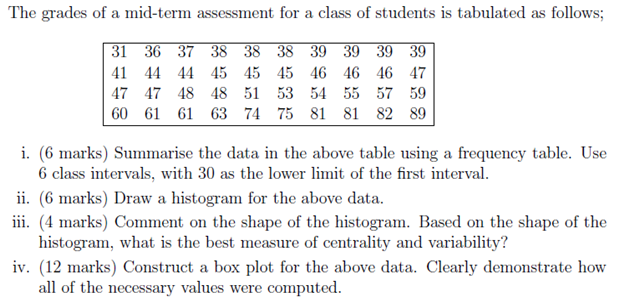
\includegraphics[width=0.9\linewidth]{Week3Boxplotquestion}
%\end{figure}

\subsection{Boxplots}
\begin{center}
	\begin{tabular}{cccccccccc}
		\hline 
		4 & 6 & 8 & 9 & 17 & 17 & 18 & 19 & 20 & 22 \\ 
		
		22 & 27 & 28 & 29 & 31 & 35 & 38 & 39 & 40 & 46 \\ 	
		48 & 56 & 56 & 57 & 57 & 58 & 58 & 60 & 61 & 62 \\ 	
		64 & 66 & 68 & 69 & 74 & 75 & 78 & 79 & 80 & 82 \\ \hline
		
	\end{tabular} 
\end{center}


lower fence?
Upper fence?

Any values above or below fences?

\newpage
\section{Tutorial C - Probability}	
\subsection*{Question 1}
Assume that there are three different routes to get to a particular location: $R_1$, $R_2$ and $R_3$. You take $R_1$ 75\% of the time, $R_2$ 20\% of the time and $R_3$ the rest of the time. If you take $R_1$, there is a 90\% chance that you will be on time; if you take $R_2$, there is a 50\% chance that you will be on time and, if you take $R_3$, there is a 70\% chance that you will be on time. \\[0.1cm]
Let $T$ represent on time.\\[-0.2cm]

{\bf(a)} If $T$ represents ``on time'', what notation would we use for ``late''? \quad {\bf(b)} What is the value of $\Pr(R_1 \cap R_2)$? \quad {\bf(c)} Calculate the probability of being on time. \quad {\bf(d)} \emph{Given that} you \emph{are} on time, calculate the probabilities of having used each of the routes. \quad {\bf(e)} Given that you are late, what is the probability that you used $R_1$?






\subsection*{Question 5}
In your favourite RPG game, let's assume that in selecting your character there are 5 character classes and 2 genders. Let's also assume there are 3 levels of difficulty for this game.\\[-0.2cm]

{\bf(a)} How many possible ways can you play this game? \quad {\bf(b)} What if you always choose the ``warrior'' class? \quad {\bf(c)} What if you always choose a female character? \quad {\bf(d)} What if you always play on the highest difficulty setting? \quad {\bf(e)} Let's assume the game has a two-player mode. How many possible ways can you play this game? (hint: you cannot play the game on different difficulty levels). {\bf(f)} What if your friend chooses a different character class to you?



\subsection*{Question 6}
Assume that you are going to an exam and you can only bring 3 items. You have the following items: $\{\text{mobile phone, } \text{pen, } \text{ruler, } \text{calculator, } \text{laptop, } \text{apple} \}$.\\[-0.2cm]

\begin{enumerate}[(i)]
\item In order to make your decision, you first \emph{arrange} these 6 items on your desk. How many possible arrangements are there? \item How many possible groups of three items can you bring with you? \item What if you decide that the pen is essential? \item What if the pen is essential and you also decide that you won't bring an apple or a laptop?
\end{enumerate}


\subsection*{Question 7}
A team of 5 people is required to perform a particular task. We are selecting from a group of 7 women and 3 men.\\[0.2cm]
How many selections are there:\\[-0.2cm]

{\bf(a)} Altogether? \quad {\bf(b)} If one of the men is an expert and must be on the team? \quad {\bf(c)} If two of the individuals do not get along and cannot be on the team together? \quad {\bf(d)} If the group must contain 3 women and 2 men? {\bf(e)} If the group must contain more women than men? \quad {\bf(f)} If the group must contain more men than women?


\section{Tutorial G - Normal Distribution}
\subsection*{Question 1}
Assume that a character in a game is programmed to have an attack power according to $X \sim \text{Normal}(\mu=40,\sigma=3)$.\\[-0.2cm]

{\bf(a)} What is the probability that the attack is greater than 45? \quad {\bf(b)} What is the probability that the attack is between 32 and 42? \quad {\bf(c)} Let $X_1$ and $X_2$ be the first and second attacks. What is the probability that the \emph{sum} of these two attacks is greater than 85 units? \quad \\{\bf(d)} Calculate 99\% limits for the sum of two attacks.  \quad {\bf(e)} What is the probability that the \emph{difference} in attacks is more than 5 units? Note that attack 2 can be 5 units more than attack 1 or attack 1 can be 5 units more than attack 2, i.e., $\Pr(|D|>5)=\Pr(D<-5) + \Pr(D>5)$.



\subsection*{Question 2}

A character in a game deals a standard attack 75\% of the time and a critical attack the rest of the time (call these events $S$ and $S^c$). Given that it is a standard attack, the attack power is $X\,|\,S \sim \text{Normal}(\mu=40,\sigma=3)$. When the character deals a critical attack, a random fluctuation is added to this according to a $\text{Normal}(\mu=5,\sigma=1)$ distribution.\\[-0.2cm]

{\bf(a)} What is the distribution of $X\,|\,S^c$? \quad {\bf(b)} Calculate $\Pr(X<43\,|\,S)$ and $\Pr(X<43\,|\,S^c)$. \quad {\bf(c)} Calculate $\Pr(X<43)$. \,\, (hint: law of total probability) \quad {\bf(d)} If the character deals less than 43 damage points, what is the probability that the attack was a critical attack?



\subsection*{Question 3}
The income of a technician (in thousands) is $X_1 \sim \text{Normal}(\mu=30,\sigma=2)$. The income of an engineer is $X_2 \sim \text{Normal}(\mu=40,\sigma=3.5)$. \\[-0.2cm]

{\bf(a)} Calculate the probability that an engineer earns more than a technician. \quad {\bf(b)} Calculate 90\% limits for the difference in their income. \quad {\bf(c)} For a group of 25 technicians, calculate the probability that the average wage is less than 30500, i.e., $\Pr(\,\overline{\!X}_1 < 30.5)$. \quad {\bf(d)} In a group of 10 engineers, what is the probability that \emph{at least two} of them earn more than 45000? (hint: binomial with $p = \Pr(X_2 > 45)$) \quad {\bf(e)} For a sample of 30 technicians and 35 engineers, calculate the 80\% limits for the difference in their average wages.


\subsection*{Question 4}
Let $X \sim \text{Exponential}(\lambda=0.02)$. Calculate the following:\\[-0.2cm]

{\bf(a)} $\Pr(\,\overline{\!X} > 55)$ in a group of 100. \quad {\bf(b)} $\Pr(\,\overline{\!X} < 53)$ in a group of 40. \quad {\bf(c)} The value of $\bar x$ such that $\Pr(\,\overline{\!X} > \bar x) = 0.1$ when $n=65$. \quad {\bf(c)} The value of $n$ if $\Pr(\,\overline{\!X} < 49) = 0.1$.



\section{KB Tutorial 3}
\subsection*{Question 1}
Assume that there are three different routes to get to a particular location: $R_1$, $R_2$ and $R_3$. You take $R_1$ 75\% of the time, $R_2$ 20\% of the time and $R_3$ the rest of the time. If you take $R_1$, there is a 90\% chance that you will be on time; if you take $R_2$, there is a 50\% chance that you will be on time and, if you take $R_3$, there is a 70\% chance that you will be on time. \\[0.1cm]
Let $T$ represent on time.\\[-0.2cm]

{\bf(a)} If $T$ represents ``on time'', what notation would we use for ``late''? \quad {\bf(b)} What is the value of $\Pr(R_1 \cap R_2)$? \quad {\bf(c)} Calculate the probability of being on time. \quad {\bf(d)} \emph{Given that} you \emph{are} on time, calculate the probabilities of having used each of the routes. \quad {\bf(e)} Given that you are late, what is the probability that you used $R_1$?






\section{KB tutorial 4}

\subsection*{Question 1}
You develop a random number generater which assigns a value to the random variable $X$ according to the following probability distribution:
\begin{center}
	\begin{tabular}{|c|ccccc|}
		\hline
		&&&&&\\[-0.4cm]
		$x$ & 0.0 & 0.5 & 1.0 & 2.0 & 3.0 \\
		\hline
		&&&&&\\[-0.4cm]
		$\Pr(X=x)$ & $0.4$ & $0.2$ & $0.15$ & $0.15$ & $?$ \\[0.1cm]
		\hline
		\multicolumn{6}{c}{}\\
	\end{tabular}
\end{center}

{\bf(a)} What is value the value of $\Pr(X = 3.0)$? \quad {\bf(b)} Calculate $E(X)$ and $Sd(X)$. \quad {\bf(c)} You produce a gambling game where the player wins (in euro) the value of $X$ generated, e.g., if a $2.0$ appears, \euro{2} is won. How much should you charge for a play of this game so that that \emph{you} (the programmer) make a profit of \euro{0.10} on average per game? (i.e., the player \emph{loses} \euro{0.10} on average) \quad {\bf(d)} Using your answer to part (c), determine the probability that you make a profit when somebody plays this game. \quad {\bf(e)} If 10 people play this game, what is the probability that you make a profit 8 times?

\subsection*{Question 2}
You flip three coins. Let $X = $ ``the number of heads'' and $Y = $ ``the number of unique faces''.\\[-0.2cm]

{\bf(a)} What is the sample space for this experiment? \quad {\bf(b)} Construct the \emph{joint distribution} for $X$ and $Y$. \quad {\bf(c)} Based on this joint distribution, construct the \emph{marginal} distribution for $X$ and for $Y$. \quad {\bf(d)} Are $X$ and $Y$ independent? \quad {\bf(e)} Calculate $E(Y)$ and $Sd(Y)$. \quad {\bf(f)} Calculate $\Pr(Y=2\,|\,X=2)$ and interpret its value (compare with $\Pr(Y=2)$).


\subsection*{Question 3}
Let $X =$ ``the attack power of player 1'' and let $Y =$ ``the attack power of player 2''.\\[-0.3cm]

Let the probability distributions for $X$ and $Y$ be:
\begin{center}
	\begin{tabular}{|c|ccc|c|c|ccc|}
		\cline{1-4}\cline{6-9}
		&&&&&&&&\\[-0.4cm]
		$x$ & 0 & 100 & 300 & \qquad\qquad & $y$ & 0 & 80 & 200\\
		\cline{1-4}\cline{6-9}
		&&&&&&&&\\[-0.4cm]
		$\Pr(X=x)$ & $0.2$ & $0.75$ & $0.05$ & & $\Pr(Y=y)$ & $0.1$ & $0.6$ & $0.3$ \\[0.1cm]
		\cline{1-4}\cline{6-9}
		%\multicolumn{9}{c}{}
	\end{tabular}
\end{center}
{\footnotesize(e.g., p1 misses 20\% of the time, deals 100 points of damage 75\% of the time and performs a critical blow 5\% of the time.)}\\[-0.2cm]

{\bf(a)} What is the average attack power of each player? \quad {\bf(b)} If both players have 1000 hit-points, how many attacks does it take for player 1 to defeat player 2 and vice versa? Which player will win on average? \quad {\bf(c)} Let's now assume that player 1 uses his/her \emph{first} turn to cast a spell (and therefore does not attack in this turn). The result of the spell is that player 2 can no longer perform a critical blow, i.e., $\Pr(Y=200) = 0$, \emph{from turn two onwards}. Since setting $p(200) = 0$ leads to $\sum p(y) \ne 1$, assume that the remaining probability ($= 0.3$) is distributed evenly between $p(0)$ and $p(80)$. What is the outcome of the battle now?


\subsection*{Question 4}

You flip a coin 10 times - let $X =$ ``the number of heads''. Using the binomial probability function, calculate the following:\\[-0.2cm]

{\bf(a)} $\Pr(X = 2)$. \quad {\bf(b)} $\Pr(X = 0)$. \quad {\bf(c)}  $\Pr(X > 2)$. \quad {\bf(d)} $\Pr(X \le 3)$. \quad {\bf(e)} $\Pr(5 \le X \le 7)$.  \quad {\bf(f)} $E(X)$ and $Sd(X)$. \quad {\bf(g)} Using the binomial tables, calculate $\Pr(X \le10)$ in the case where the coin is flipped 20 times. \quad {\bf(h)} If the coin is flipped 50 times, what is $E(X)$?

\subsection*{Question 5}

Repeat Question 4 (a) - (e) but now using the binomial tables.



\subsection*{Question 6}

Let's assume that a sequence of bits (binary numbers) is transmitted and, at the other end, decoded; the decoder has a 10\% chance reading a bit incorrectly (i.e., reading a 0 as 1 or vice versa). Let $X$ be the number of errors in the sequence received (i.e., the decoded sequence). Calculate the probability that there are: \\[-0.2cm]

{\bf(a)} \emph{No} errors in a 20-bit string. \quad {\bf(b)} Less than three errors in a 10-bit string. \quad {\bf(c)} More than 10 errors in (i) a 50-bit string and (ii) a 100-bit string (hint: use tables). \quad {\bf(d)} Calculate the average number of errors in a 100-bit string. Calculate the standard deviation also.


\subsection*{Question 7}
We follow on from Question 6 but now consider the case where, to reduce the probability of error, each bit is sent \emph{three} times and then a ``majority vote'' approach is used to determine the value of each received bit. The following example explains the situation:\\[-0.5cm]
\begin{center}
	\begin{tabular}{ccccc}
		\hline
		&&&&\\[-0.3cm]
		\multirow{2}{*}{Sent} & $0$ & $1$ & $1$ & $0$ \\
		& $\overbrace{000}$ & $\overbrace{111}$ & $\overbrace{111}$ & $\overbrace{000}$ \\[0.2cm]
		\hline
		&&&&\\[-0.3cm]
		\multirow{2}{*}{Received} & $\underbrace{001}$ & $\underbrace{111}$ & $\underbrace{010}$ & $\underbrace{000}$ \\
		& $0$ & $1$ & $0$ & $0$ \\[0.2cm]
		\hline
		%\multicolumn{5}{c}{}
	\end{tabular}
\end{center}
$\Rightarrow$ there is one error in decoding the first $000$, but since the majority result is taken, this bit is correctly identified as a $0$. There are two errors in decoding the second $111$, so this bit is misread as a $0$. It is clear that a character is misread if the decoder makes \emph{two or three errors} in these blocks of three replicates.\\[-0.2cm]

{\bf(a)} Show that sending each bit 3 times reduces the error probability from 10\% to 2.8\%. \quad\\ {\bf(b)} Using this reduced value, $p=0.028$, calculate the probability that there are no errors in a 20-bit string. Compare this result to Q6(a). \quad {\bf(c)} Now assume that each bit is sent 5 times and, again, the majority vote approach is used. Calculate the probability that there are no errors in a 20-bit string in this case. %\quad {\bf(d)} Recalculate the two probabilities from part (c) using the Poisson approximation.

\newpage
\section{KB Tutorial 6}






\subsection*{Question 4}
{\footnotesize({\bf Note}: this is not a queueing theory question. It is a generalisation of a question which appears on Tutorial2)}\\[0.1cm]
There are two possible routes to a particular location. You take $R_1$ 80\% of the time and $R_2$ 20\% of the time. We assume that travel time has an exponential distribution and, furthermore, the average travel time is 0.25 hours if you take $R_1$ and 0.5 hours if you take $R_2$.\\[-0.2cm]

{\bf(a)} Calculate the probability that the journey takes more than 0.5 hours for each of the routes, i.e., $\Pr(T > 0.5\,|\,R_1)$ and $\Pr(T > 0.5\,|\,R_2)$ respectively. \quad {\bf(b)} Calculate $\Pr(T > 0.5)$. (hint: law of total probability) \quad {\bf(c)} Given that $T>0.5$ hours, what is the probability that you used $R_1$? (i.e., calculate $\Pr(R_1\,|\,T>0.5)$) \quad {\bf(d)} Derive a general expression for $\Pr(R_1\,|\,T>t)$ and evaluate it at $t=0.25$, $t = 1$ and $t = 2$ respectively. Interpret the results.




\subsection*{Question 5}
Let $X \sim \text{Normal}(\mu=10,\sigma=2)$. Calculate the following:\\[-0.2cm]

{\bf(a)} $\Pr(X>10)$. \quad {\bf(b)} $\Pr(X<3)$. \quad {\bf(c)} $\Pr(X>8.4)$. \quad {\bf(d)} $\Pr(6<X<14)$. \quad {\bf(e)} The value of $x$ such that $\Pr(X>x)$ = 0.3. \quad {\bf(f)} The value of $x$ such that $\Pr(X>x)$ = 0.8.



\subsection*{Question 6}
Assume that speeds of cars on a motorway have a normal distribution with mean 115km/hr and standard deviation 4km/hr.\\[-0.2cm]

{\bf(a)} Draw a rough sketch of the distribution. \quad {\bf(b)} $\Pr(X>120)=$ ? \quad {\bf(c)} $\Pr(X<100)=$ ? \quad {\bf(d)} $\Pr(100<X<110)=$ ? \quad {\bf(e)} 1\% of drivers travel above what speed?







\subsection*{Question 7}
For \emph{any} normal variable $X \sim \text{Normal}(\mu,\sigma)$:\\[-0.2cm]

{\bf(a)} Show that $\Pr(\mu-3\,\sigma<X<\mu+3\,\sigma) = 0.997$. \quad {\bf(b)} Find a value for $k$ such that $\Pr(\mu-k\,\sigma<X<\mu+k\,\sigma) = 0.95$. \quad {\bf(c)} Find $k$ such that $\Pr(\mu-k\,\sigma<X<\mu+k\,\sigma) = 0.99$. \quad {\bf(d)} Show that $\Pr(X>\mu+1.64\,\sigma) = 0.05.$







\end{document} 
